
% Tệp mẫu làm đề thi trắc nghiệm dựa vào gói lệnh dethi.sty 3.2
% Tác giả: Nguyên Hữu Điển
% Khoa Toán Cơ Tin học, ĐHKHTN HN, ĐHQGHN
% 334, Nguyễn Trãi, Thanh Xuân, Hà Nội
% huudien@vnu.edu.vn
% Ngày 26/12/2009
%%%%%%%%%%%%%%%%%%%%%%%%%%%%

\documentclass[12pt,openany]{article}
\usepackage{amsmath,amsxtra,amssymb,latexsym, amscd,amsthm}
\usepackage{graphicx}
\usepackage{picinpar}
\usepackage{tikz}
\usetikzlibrary{arrows}
\usepackage{tkz-tab}
\usepackage[utf8]{vietnam}
\usepackage{longtable}%
\usepackage{multicol}%
\usepackage{color}
 \usepackage{shortlst}
\usepackage{enumerate}
%%%%%%%%%%%%%%%%%%%%%
\usepackage{mathpazo} 
\voffset=-2cm
% \hoffset=-2cm
\textheight 24truecm 
\textwidth 18truecm 
\usepackage[baitap]{dethi}
\tentruong{ĐẠI HỌC KHOA HỌC TỰ NHIÊN}
\tenkhoa{Khoa Toán - Cơ -Tin học}
\loaidethi{Đề gồm có \pageref{LastPage} trang}%{ĐỀ THI LẠI}%%{ĐỀ CHÍNH THỨC}
\tenkythi{ĐỀ THI GIỮA KỲ NĂM HỌC 2016-2017}
\tenmonhoc{Môn: Toán học tính toán}
\madethi{100}
\thoigian{\underline{Thời gian làm bài: 90 phút, không kể thời gian phát đề}}   
\hovaten{Họ và tên}         %Nếu không muốn có dòng này không gõ lệnh
\tenlop{Tên lớp}         %Nếu không muốn có dòng này không gõ lệnh
\sobaodanh{Số báo danh}  %Nếu không muốn có dòng này không gõ lệnh
\daungoac{\cboxx}{}
\khoanh{\cboxv}
\chuphuongan{\small\bfseries\Alph}
\mauchu{blue}
\PSNrandseed{\time}
% \coloigiai
\usepackage{centerpage}
\usepackage{lastpage}
\graphicspath{{hinh-cauhoi/}} 
\parindent 20pt

\begin{document}

\lamtieude
\indebai
\loadrandomproblems[bttracnghiem]{40}{vd03-cauhoi-toan-baitracnghiem}



\baitracnghiem{t2017:b01}{%
Đường cong trong hình bên là đồ thị của một hàm số trong 
\begin{window}[0,r,{\hspace*{1cm}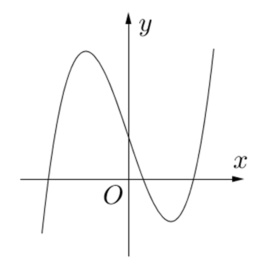
\includegraphics[scale=0.6]{toan01}\hspace*{1cm}},{\label{fig:b01}}]
bốn hàm số được liệt kê ở bốn phương án $A, B, C, D$ dưới
đây.  Hỏi hàm số đó là hàm số nào ?
\end{window}
}{
\datcot[4]
\bonpa
{\sai{$y=-x^2+x-1$.}}
{\sai{$y=-x^3+3x+1$.}}
{\dung{$y=x^3-3x+1$.}}
{\sai {$y=x^4-x^2+1$.}}
\loigiai{ 
Dựa vào đồ thị hàm số ta loại đi 2 đáp án A và C.\\
Dựa vào đồ thị hàm số ta suy ra bảng biến thiên của hàm số có dạng\\
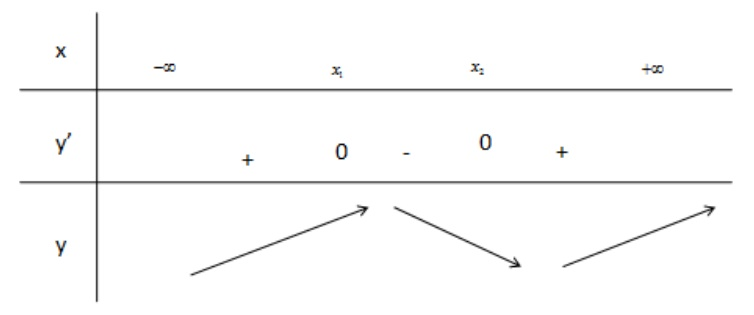
\includegraphics[scale=0.5]{gtoan01}\\
Như vậy ta thấy $y’ = 0$ có 2 nghiệm phân
 biệt và $y’$ trái dấu với hệ số của a nên hệ số $a > 0$
}
}

\baitracnghiem{t2017:b02}{%
Cho hàm số $y=f(x)$ có  $\lim\limits_{x\rightarrow +\infty}f(x)=1$ và   $\lim\limits_{x\rightarrow -\infty}f(x)=-1$. Khẳng định nào sau
đây là khẳng định đúng ?
}{
\datcot[4]
\bonpa
{\sai{Đồ thị hàm số đã cho không có tiệm cận ngang.}}
{\sai{Đồ thị hàm số đã cho có đúng một tiệm cận ngang.}}
{\dung{Đồ thị hàm số đã cho có hai tiệm cận ngang là các đường thẳng  $y=1$ và  $y=-1$.}}
{\sai{Đồ thị hàm số đã cho có hai tiệm cận ngang là các đường thẳng $x=1$ và  $x=-1$.}}
\loigiai{
Vì  $\lim\limits_{x\rightarrow\infty} f(x)=1$ nên hàm số có tiệm cận ngang $y = 1$\\
Vì  $\lim\limits_{x\rightarrow-\infty} f(x)=1$ nên hàm số có tiệm cận ngang $y =-1$\\
Vậy hàm số có 2 tiệm cận ngang.
}
}

\baitracnghiem{t2017:b03}{%
 Hỏi hàm số $y=2x^4+1$  đồng biến trên khoảng nào ?
}{
\datcot
\bonpa
{\sai{$\left(-\infty; -\dfrac{1}{2}\right)$.}}
{\dung{$\left(0;+\infty\right)$.}}
{\sai{$\left(-\dfrac{1}{2}; +\infty\right)$.}}
{\sai {$(-\infty;0)$.}}
\loigiai{
$y=2x^4+1\Rightarrow y'=8x^3$.\\
Với $x\in (0,\; +\infty)\Rightarrow y'>0 \Rightarrow $ Hàm số đồng biến trên $(0; +\infty)$
}
}

\baitracnghiem{t2017:b04}{%
Cho hàm số  $y=f(x)$ xác định, liên tục trên $\mathbb{R}$ và có bảng biến thiên :
\begin{center}
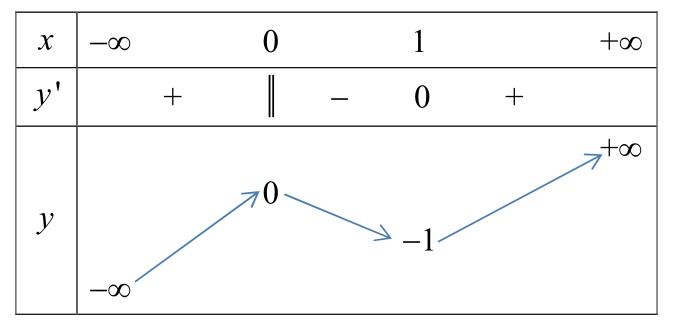
\includegraphics[scale =0.5]{toan02}
\end{center}
Khẳng định nào sau đây là khẳng định đúng ?
}{
\datcot[4]
\bonpa
{\sai{Hàm số có đúng một cực trị.}}
{\sai{Hàm số có giá trị cực tiểu bằng $1$.}}
{\sai {Hàm số có giá trị lớn nhất bằng $0$ và giá trị nhỏ nhất bằng  $1$.}}
{\dung{Hàm số đạt cực đại tại  $x=0$ và đạt cực tiểu tại  $x=1$.}}
\loigiai{Hàm số đạt cực đại tại  $x=0$ và đạt cực tiểu tại  $x=1$.
}
}

\baitracnghiem{t2017:b05}{%
Tìm giá trị cực đại $y_{\mbox{\scriptsize  \textit{CĐ} }}$ của hàm số $y=x^3-3x+2$.
}{
\datcot
\bonpa
{\dung{$y_{\mbox{\scriptsize \textit{CĐ} }}=4$.}}
{\sai{$y_{\mbox{\scriptsize \textit{CĐ} }}=1$.}}
{\sai{$y_{\mbox{\scriptsize  \textit{CĐ} }}=0$.}}
{\sai {$y_{\mbox{\scriptsize \textit{CĐ} }}=-1$.}}
\loigiai{
Ta có $y=x^3-3x+2$; $y'=3x^2-3$; $y'=0 \Leftrightarrow x=\pm 1$.\\
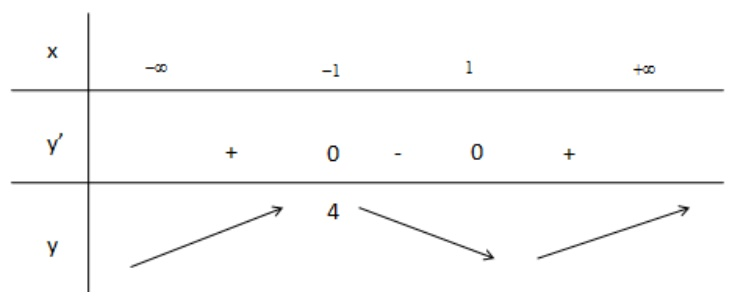
\includegraphics[scale=0.5]{gtoan02}\\
}
}

\baitracnghiem{t2017:b06}{%
Tìm giá trị nhỏ nhất của hàm số $y=\dfrac{x^2+3}{x-1}$ trên đoạn $[2;4]$.
}{
\datcot
\bonpa
{\dung{$\min_{[2;4]} y=6$.}}
{\sai{$\min_{[2;4]} y=-2$.}}
{\sai{$\min_{[2;4]} y=-3$.}}
{\sai {$\min_{[2;4]} y=\dfrac{19}{3}$.}}
\loigiai{
 $y=\dfrac{x^2+3}{x-1}$.\\
$y'=\dfrac{2x(x-1)-x^2-3}{(x-1)^2}=\dfrac{x^2-2x-3}{(x-1)^2}$.\\
$y'=0\Leftrightarrow\left[\begin{matrix}
x=-1\quad \mbox{ loại }\\ 
x=3\quad \mbox{ thỏa mãn }\\ 
\end{matrix}\right.$.\\
Có $y(2)=7; y(3)=6; y(4)=\dfrac{19}{3} \Rightarrow \min\limits_{[2;4]} y=6$.
}
}


% \begin{enumerate}[label=\textcolor{blue}{\bf Câu \arabic*.}] 
%  \useproblem{t2017:b01}
%  \useproblem{t2017:b02}
%  \useproblem{t2017:b03}
%  \useproblem{t2017:b04}
%  \useproblem{t2017:b05}
%  \useproblem{t2017:b06}
% \end{enumerate}

\begin{enumerate}[]
 \item \causo\useproblem{t2017:b01}
 \item \causo\useproblem{t2017:b02}
 \item \causo\useproblem{t2017:b03}
 \item \causo\useproblem{t2017:b04}
 \item \causo\useproblem{t2017:b05}
 \item \causo\useproblem{t2017:b06}
\end{enumerate}

\end{document}
